\documentclass[11pt,a4paper]{article}
\usepackage[margin=2.4cm]{geometry}
\usepackage{ctex}
\usepackage{amsmath,amssymb}
\usepackage{graphicx}
\usepackage{booktabs}
\usepackage{array}
\usepackage{caption}
\usepackage{xcolor}
\usepackage{titlesec}
\usepackage[colorlinks=true,linkcolor=black,citecolor=black,urlcolor=blue!60!black]{hyperref}
\titleformat{\section}{\large\bfseries\color{black!85}}{\thesection}{0.6em}{}
\titleformat{\subsection}{\normalsize\bfseries\color{black!70}}{\thesubsection}{0.5em}{}
\captionsetup{font=small,labelfont=bf,labelsep=period}
\setlength{\parskip}{3pt}\setlength{\parindent}{0pt}
\renewcommand{\abstractname}{\bfseries 摘\ 要}

\title{\bfseries 可重复使用火箭喷管壁的多物理场耦合与老化损伤稀疏辨识:\\[2pt]\large 交互项挖掘与未知常数的 SINDy-PI 辨识}
\date{}

\begin{document}
\maketitle

\begin{abstract}
\noindent 可重复使用火箭喷管壁的结构损伤由多物理场（温度、应力、氧分压）驱动，且氧化、疲劳、蠕变等机制间存在非线性交互。本文以圆台（喷管状）轴对称壁为计算域，建立单向耦合前向模型，在其中种入已知交互项与已知常数作为真值，用物理信息稀疏辨识（SINDy）挖掘耦合项，并用 SINDy-PI 辨识真实场景下不可靠已知的活化能与幂指数。结果表明：(i) 无噪声下，多项耦合交互（温度相关氧扩散、应力调制氧扩散、应力助氧化、氧化–疲劳、氧化–蠕变）支持均被正确识别、无误选、系数恢复误差 $\le 4\%$；EIV 噪声下交互项系数误差随噪声单调增大，含拉普拉斯算子的场×场项较损伤×损伤项更敏感；(ii) 仿真深化至损伤中后期非线性区后，SINDy-PI 的 profile 扫描从数据辨识出 $E_{a,d},E_{a,h},E_{a,o},E_{a,c}$ 与 Paris $m,q$、Norton $n$（全部命中真值）。本研究为方法可行性验证。
\end{abstract}

\section{引言}
可重复使用运载火箭（RLV）喷管壁在多次点火中承受高温、应力与氧化环境的耦合作用，其结构损伤评估是复用可靠性的核心问题。多物理场之间的耦合作用是该问题的最大难点；损伤演化内部亦存在机制间的非线性交互，不宜以简单线性叠加处理。更甚者，控制方程中的活化能 $E_a$（在 $e^{-E_a/RT}$ 指数内）、Paris 指数 $m$ 与饱和指数 $q$、Norton 指数 $n$ 等常数在真实场景里随材料/工况而变、并不可靠已知，且它们均非线性于参数，标准 SINDy（线性可分）无法处理。

本文针对"耦合项挖掘"与"未知常数辨识"两类问题，分别用 SINDy 与 SINDy-PI，在已知答案的合成圆台场上检验框架可行性。本文为方法可行性验证，控制律为自设已知真值，非真实机理发现。

\section{研究方法}

\subsection{耦合前向模型与自设控制方程}
以圆台（喷管状）轴对称薄壳（壁厚 $h_{wall}=5$~mm、轴向 $30$ 节点、$10$ 层厚）为计算域 $\Omega$。因 $h_{wall}/r\approx 3\%$--$10\%\ll 1$ 取薄壳近似，空间扩散用二维 $\partial_r^2+\partial_z^2$（曲率项 $(1/r)\partial_r$ 为 $O(h_{wall}/r)$ 小量，略）。建模约定：\textbf{物理场与损伤不反向耦合}——物理场由边界条件与场×场交互驱动演化，损伤由物理场单向算出。温度场与氧分压场用隐式 backward Euler 求解，应力为准静态代数本构，四类损伤前向 Euler 积分。统一记号 $\mathrm{arr}_{E_a}(T)=e^{-E_a/RT}$。自设控制方程如下（$F$ 为基本机制项，$g$ 为交互耦合项）：

\textbf{温度场}（域内 PDE + 边界条件，表面热流以 Robin 条件施加，不混入域内方程）：
\begin{align*}
&\text{域内:}\quad \partial T/\partial t=\alpha\nabla^2 T,\quad (r,z)\in\Omega\\
&\text{内壁:}\ -k\,\partial T/\partial n=h_g(T_{gas}-T);\qquad
 \text{外壁:}\ -k\,\partial T/\partial n=\varepsilon\sigma_{SB}(T^4-T_{amb}^4);\quad
 \text{轴向端:}\ \partial T/\partial z=0
\end{align*}

\textbf{氧分压场}（内壁 Dirichlet $p_{O_2}|_\text{内}=p_{O_2,gas}$）：
\begin{equation*}
\frac{\partial p_{O_2}}{\partial t}=\big[\underbrace{D_0\,\mathrm{arr}_{E_{a,d}}(T)}_{g(T\to p_{O_2})}+\underbrace{\lambda\sigma}_{g(\sigma\to p_{O_2})}\big]\nabla^2 p_{O_2}
\end{equation*}

\textbf{应力}（准静态代数本构）。$\kappa\in(0,1]$ 为薄壳机械约束因子（$\kappa=1$ 完全约束、$\kappa<1$ 部分松弛，本文取 $\kappa=0.40$）：
\begin{equation*}
\sigma=\underbrace{\kappa\,\frac{E\alpha_{th}}{1-\nu}(T-T_m)}_{g(T\to\sigma)}+\underbrace{\frac{p\,r_{in}}{h_{wall}}}_{g(p\to\sigma)}
\end{equation*}

\textbf{损伤演化}（$F$ 机制律 + $g$ 交互项；热疲劳按循环 $N$ 的 Paris 律换算为连续速率 $dD_f/dt=(dD_f/dN)/T_c$，$T_c$ 循环周期，$\Delta\sigma$ 为每循环应力幅）：
\begin{align*}
dD_h/dt &= \underbrace{a_h\,\mathrm{arr}_{E_{a,h}}(T)}_{F}\\
dD_o/dt &= \underbrace{a_o\,\mathrm{arr}_{E_{a,o}}(T)\,p_{O_2}}_{F}+\underbrace{a_{os}\,\mathrm{arr}_{E_{a,o}}\,p_{O_2}\,\sigma}_{g}+\underbrace{a_{of}\,\mathrm{arr}_{E_{a,o}}\,p_{O_2}\,D_f}_{g}\\
dD_f/dt &= \underbrace{a_f(\Delta\sigma)^m(1-D_f)^{-q}/T_c}_{F}+\underbrace{a_{fo}(\Delta\sigma)^m D_o/T_c}_{g}\\
dD_c/dt &= \underbrace{a_c|\sigma|^n\,\mathrm{arr}_{E_{a,c}}(T)}_{F}+\underbrace{a_{co}|\sigma|^n\,\mathrm{arr}_{E_{a,c}}\,D_o}_{g}
\end{align*}
\textbf{总损伤}取非加性（weakest-link）组合以保证 $D_{total}\le 1$：
\begin{equation*}
D_{total}=1-\prod_{k\in\{h,o,f,c\}}(1-D_k)
\end{equation*}
其中 $E_{a,d},E_{a,h},E_{a,o},E_{a,c},m,n,q$ 为真实场景不可靠已知的非线性于参数常数，由 SINDy-PI 辨识（非文献假定）。仿真取 $15$ 个热循环，使各损伤进入 $0.3$–$0.5$ 的中后期非线性区。\textbf{先验与辨识边界：}导热扩散率 $\alpha=k/(\rho c_p)$、应力代数本构参数（$E,\alpha_{th},\nu,\kappa$）与边界换热/辐射系数取作已知物理先验固定（材料物性/成熟定律，不予辨识）；SINDy 辨识 $p_{O_2}$ 与四类损伤方程的基项及交互项系数（含 $a_h,a_o,a_f,a_c$），SINDy-PI 辨识非线性常数 $E_a,m,q,n$。

\subsection{稀疏辨识与 SINDy-PI}
\textbf{结构辨识（SINDy）}：候选库分双库——物理场库 $\Theta_{\mathrm{phys}}$ 与损伤库 $\Theta_{\mathrm{dmg}}$，各库内部按 $F$（基本项）与 $G$（交互项）分组。对每目标导数，用序贯阈值最小二乘（STLSQ）选稀疏支持；列按标准差缩放、不中心化，系数换算回原始尺度 $\xi_j=(\sigma_y/\sigma_j)\beta_j$。时间导数用 Savitzky--Golay 平滑求导。

\textbf{常数辨识（SINDy-PI）}：$E_a$、$m,n,q$ 位于指数/幂次的非线性参数，标准 SINDy 无法处理。直接离散成多列候选会因 $\exp(-E_{a,k}/RT)$ 各列高度共线而失效（条件数 $\gg 10^4$）。故采用 profile 扫描：对每个候选参数值做线性内层拟合、取 $R^2$ 峰值，即对非线性参数的一维/二维搜索加线性内层（疲劳的 $m,q$ 与蠕变的 $n,E_{a,c}$ 用二维扫描）。噪声检验采用 errors-in-variables（EIV）：测量噪声加到 $T,\sigma,p_{O_2}$ 与各损伤量上。

\section{结果与分析}

\subsection{挖掘出的耦合交互项}
表~\ref{tab:inter} 列出从合成场成功识别的交互项。无噪声下支持 $100\%$ 命中、$0$ 误选，各项系数恢复误差均 $\le 4\%$。第~1、2 项为场×场交互（温度相关与应力调制氧扩散），第~3--6 项为损伤×损伤或场$\to$损伤交互，对应“损伤非简单相加”。需强调：足够细的时间采样是系数精确恢复的前提——粗采样下 Savitzky--Golay 求导偏差会被共因子 $\mathrm{arr}\cdot p_{O_2}$ 不均等地摊到各交互系数上（小系数项尤甚）；本文取 $\Delta t{=}0.2$~s。

\begin{table}[h]\centering\small
\caption{成功挖掘的交互项。$\mathrm{arr}_{E_a}(T)=e^{-E_a/RT}$。}
\label{tab:inter}
\begin{tabular}{>{\raggedright\arraybackslash}p{3.0cm} >{\raggedright\arraybackslash}p{2.1cm} >{\raggedright\arraybackslash}p{2.0cm} >{\raggedright\arraybackslash}p{4.5cm} >{\raggedright\arraybackslash}p{2.3cm}}
\toprule
交互项 & 涉及物理量 & 所在方程 & 耦合机制 & 恢复系数 vs 真值 \\
\midrule
$\mathrm{arr}_{E_{a,d}}\!\cdot\!\nabla^2 p_{O_2}$ & $T\!\leftrightarrow\!p_{O_2}$ & $\partial p_{O_2}/\partial t$ & 温度相关氧扩散 & $2.89\!\times\!10^{-5}$ vs $3.0\!\times\!10^{-5}$ \\
$\sigma\!\cdot\!\nabla^2 p_{O_2}$ & $\sigma\!\to\!p_{O_2}$ & $\partial p_{O_2}/\partial t$ & 应力调制氧扩散 & $2.02\!\times\!10^{-11}$ vs $2.0\!\times\!10^{-11}$ \\
$\mathrm{arr}\!\cdot\!p_{O_2}\!\cdot\!\sigma$ & $\sigma\!\to\!D_o$ & $dD_o/dt$ & 应力助氧化\textsuperscript{1} & $0.0097$ vs $0.01$ \\
$\mathrm{arr}\!\cdot\!p_{O_2}\!\cdot\!D_f$ & $D_f\!\to\!D_o$ & $dD_o/dt$ & 疲劳裂纹露新面$\to$加速氧化 & $6.22$ vs $6$ \\
$\mathrm{Paris}\!\cdot\!D_o$ & $D_o\!\to\!D_f$ & $dD_f/dN$ & 氧化致脆$\to$加速疲劳\textsuperscript{1} & $2.25\!\times\!10^{-11}$ vs $2.25\!\times\!10^{-11}$ \\
$\mathrm{Norton}\!\cdot\!D_o$ & $D_o\!\to\!D_c$ & $dD_c/dt$ & 氧化改变蠕变\textsuperscript{2} & $6.08\!\times\!10^{-4}$ vs $6.0\!\times\!10^{-4}$ \\
\bottomrule
\end{tabular}
\end{table}

\subsection{辨识精度与噪声鲁棒性}
机制基项系数亦从数据一并恢复（$a_h\approx 900$、$a_o\approx 3.0$、$a_f\approx 1.5\!\times\!10^{-11}$、$a_c\approx 8\!\times\!10^{-4}$，误差均 $\le 0.7\%$），非真项（含 $dD_h/dt$ 的 $\mathrm{arr}_h\sigma$、$dD_f/dt$ 的 $\mathrm{Paris}\,D_c$ 等）被剔除，$R^2\approx 0.999$--$1.000$。EIV 噪声下，固定阈值 STLSQ 的支持恢复在小系数项上随噪声非单调抖动（阈值边缘的数值伪影，非物理），故以“真实支持上 OLS 的系数相对误差”为鲁棒性指标：该误差随噪声单调增大——损伤×损伤项在 $\le 5\%$ 噪声下仍 $\lesssim 5\%$，而含拉普拉斯算子的场×场扩散项因算子放大观测噪声而显著更敏感（$5\%$ 噪声即 $\sim 18\%$）（图~\ref{fig:rec}）。

\begin{figure}[h]\centering
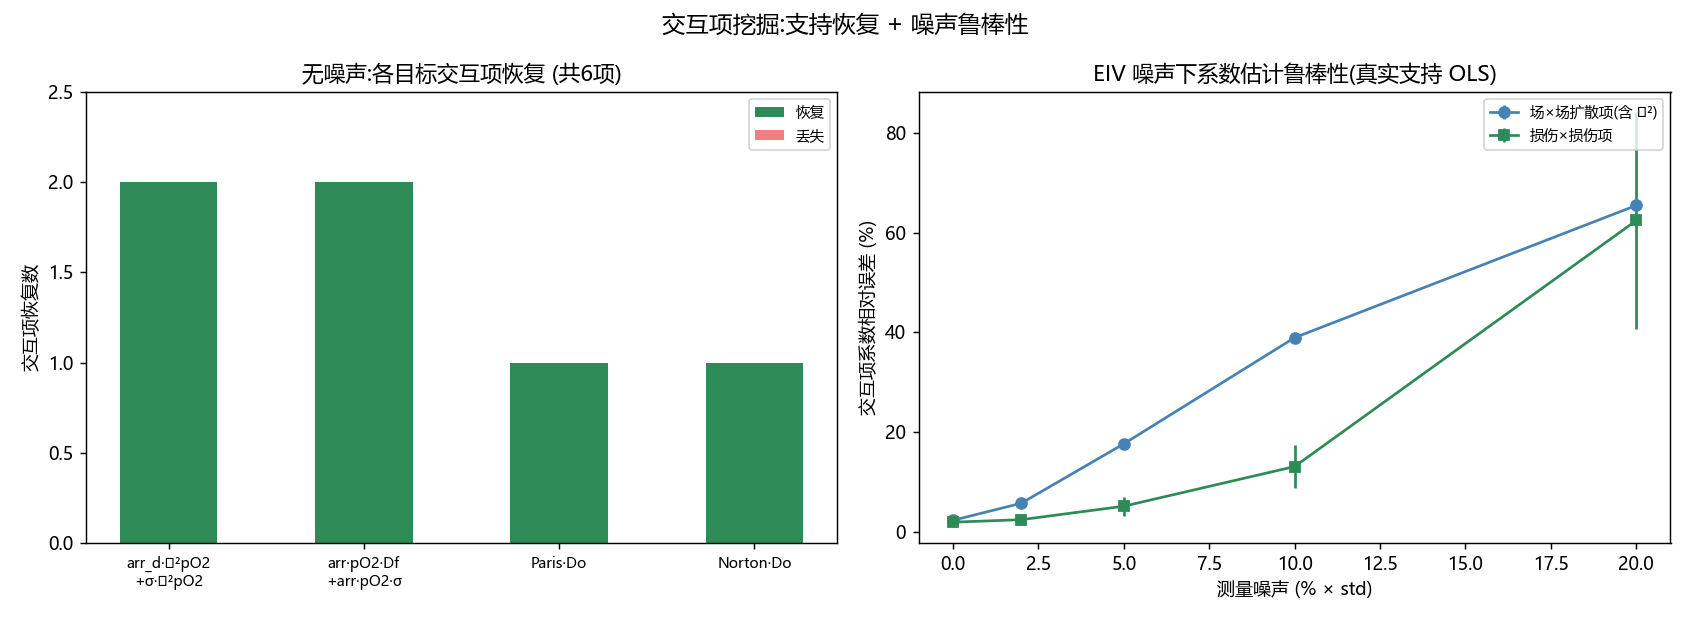
\includegraphics[width=0.85\linewidth]{figrec.png}
\caption{无噪声交互项支持恢复（左）与 EIV 噪声下交互项系数相对误差（右，按类；真实支持 OLS）。}\label{fig:rec}
\end{figure}

\subsection{未知常数的 SINDy-PI 辨识}
真实场景下 $E_a$、$m,n,q$ 不可靠已知。profile 扫描的 $R^2$-参数曲线在真值处 sharply peaked（图~\ref{fig:spi}），辨识结果全部命中真值（表~\ref{tab:spi}）。需强调：饱和指数 $q$ 在早期短时仿真（$D_f<0.1$、$(1-D_f)^{-q}\approx 1$）下不可辨；将仿真深化至损伤中后期（$D_f\approx 0.4$，进入 $(1-D_f)^{-q}$ 非线性加速区）后，$q$ 亦变得可辨——这正说明该方法对深层非线性参数的辨识能力依赖于数据是否覆盖非线性阶段。

\begin{table}[h]\centering\small
\caption{SINDy-PI 辨识的非线性于参数常数（真值对辨识隐藏）。}
\label{tab:spi}
\begin{tabular}{lccl}
\toprule
常数（单位） & 真值 & SINDy-PI 辨识 & 峰值 $R^2$ \\
\midrule
$E_{a,d}$\,(pO2 扩散, kJ/mol) & 100 & \textbf{100} & 0.998 \\
$E_{a,h}$\,(热老化, kJ/mol) & 200 & \textbf{200} & 0.999 \\
$E_{a,o}$\,(氧化, kJ/mol) & 120 & \textbf{120} & 0.999 \\
$E_{a,c}$\,(蠕变, kJ/mol) & 280 & \textbf{280} & 0.997 \\
$m$\,(Paris 疲劳指数) & 3 & \textbf{3} & 0.999 \\
$q$\,(Paris 饱和指数) & 1 & \textbf{1} & 0.999 \\
$n$\,(Norton 蠕变指数) & 4 & \textbf{4} & 0.997 \\
\bottomrule
\end{tabular}
\end{table}

\begin{figure}[h]\centering
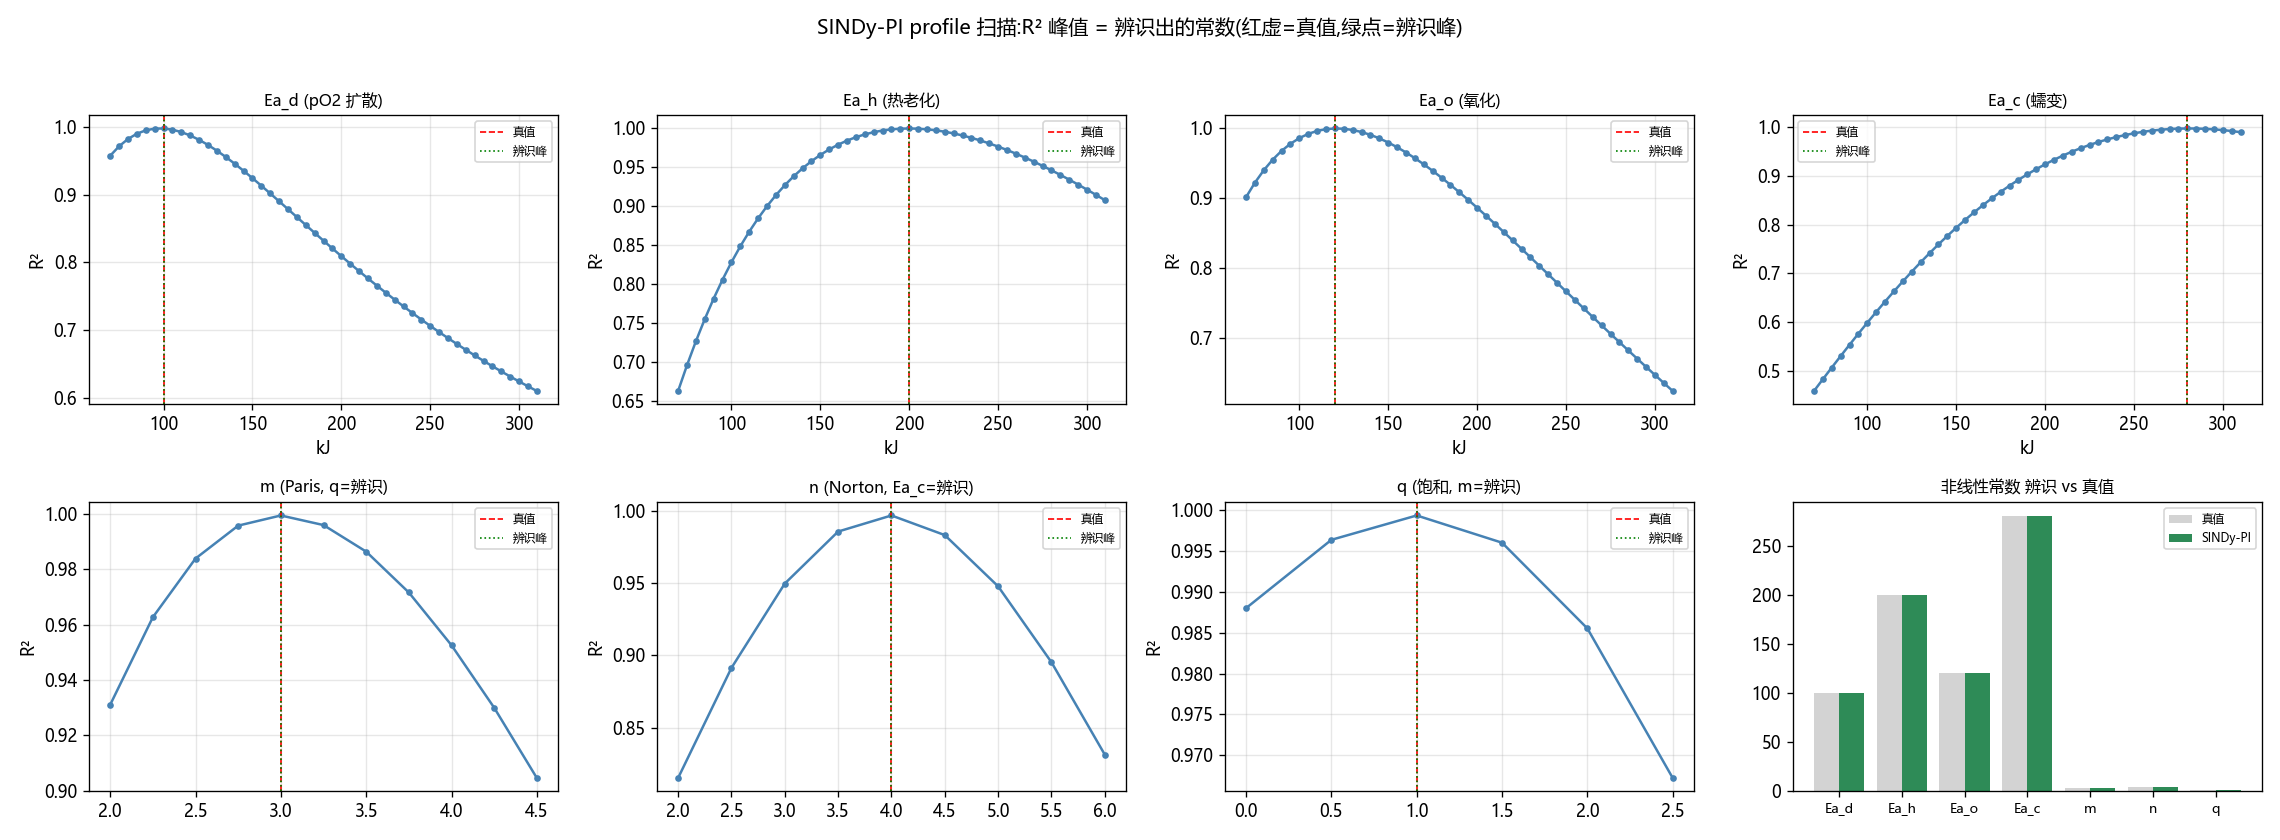
\includegraphics[width=\linewidth]{fig_sindypi.png}
\caption{SINDy-PI profile 扫描的 $R^2$-参数曲线：红虚=真值，绿点=辨识峰。各常数 $R^2$ 在真值处 sharply peaked（辨识命中）。右下：辨识值 vs 真值。}\label{fig:spi}
\end{figure}

\subsection{多物理场与损伤场的空间分布}
图~\ref{fig:3d} 把温度、应力、氧分压与四类损伤及总损伤以 3D 切口圆台呈现（上排物理场峰值时刻，下排损伤终时刻；切口面显壁厚方向分布）。深化仿真后各损伤达中后期（$D_f\approx0.4$、$D_{total}\approx0.8$），内壁喉部温度最高、气侧损伤最大，符合喷管壁的物理图景。

\begin{figure}[h]\centering
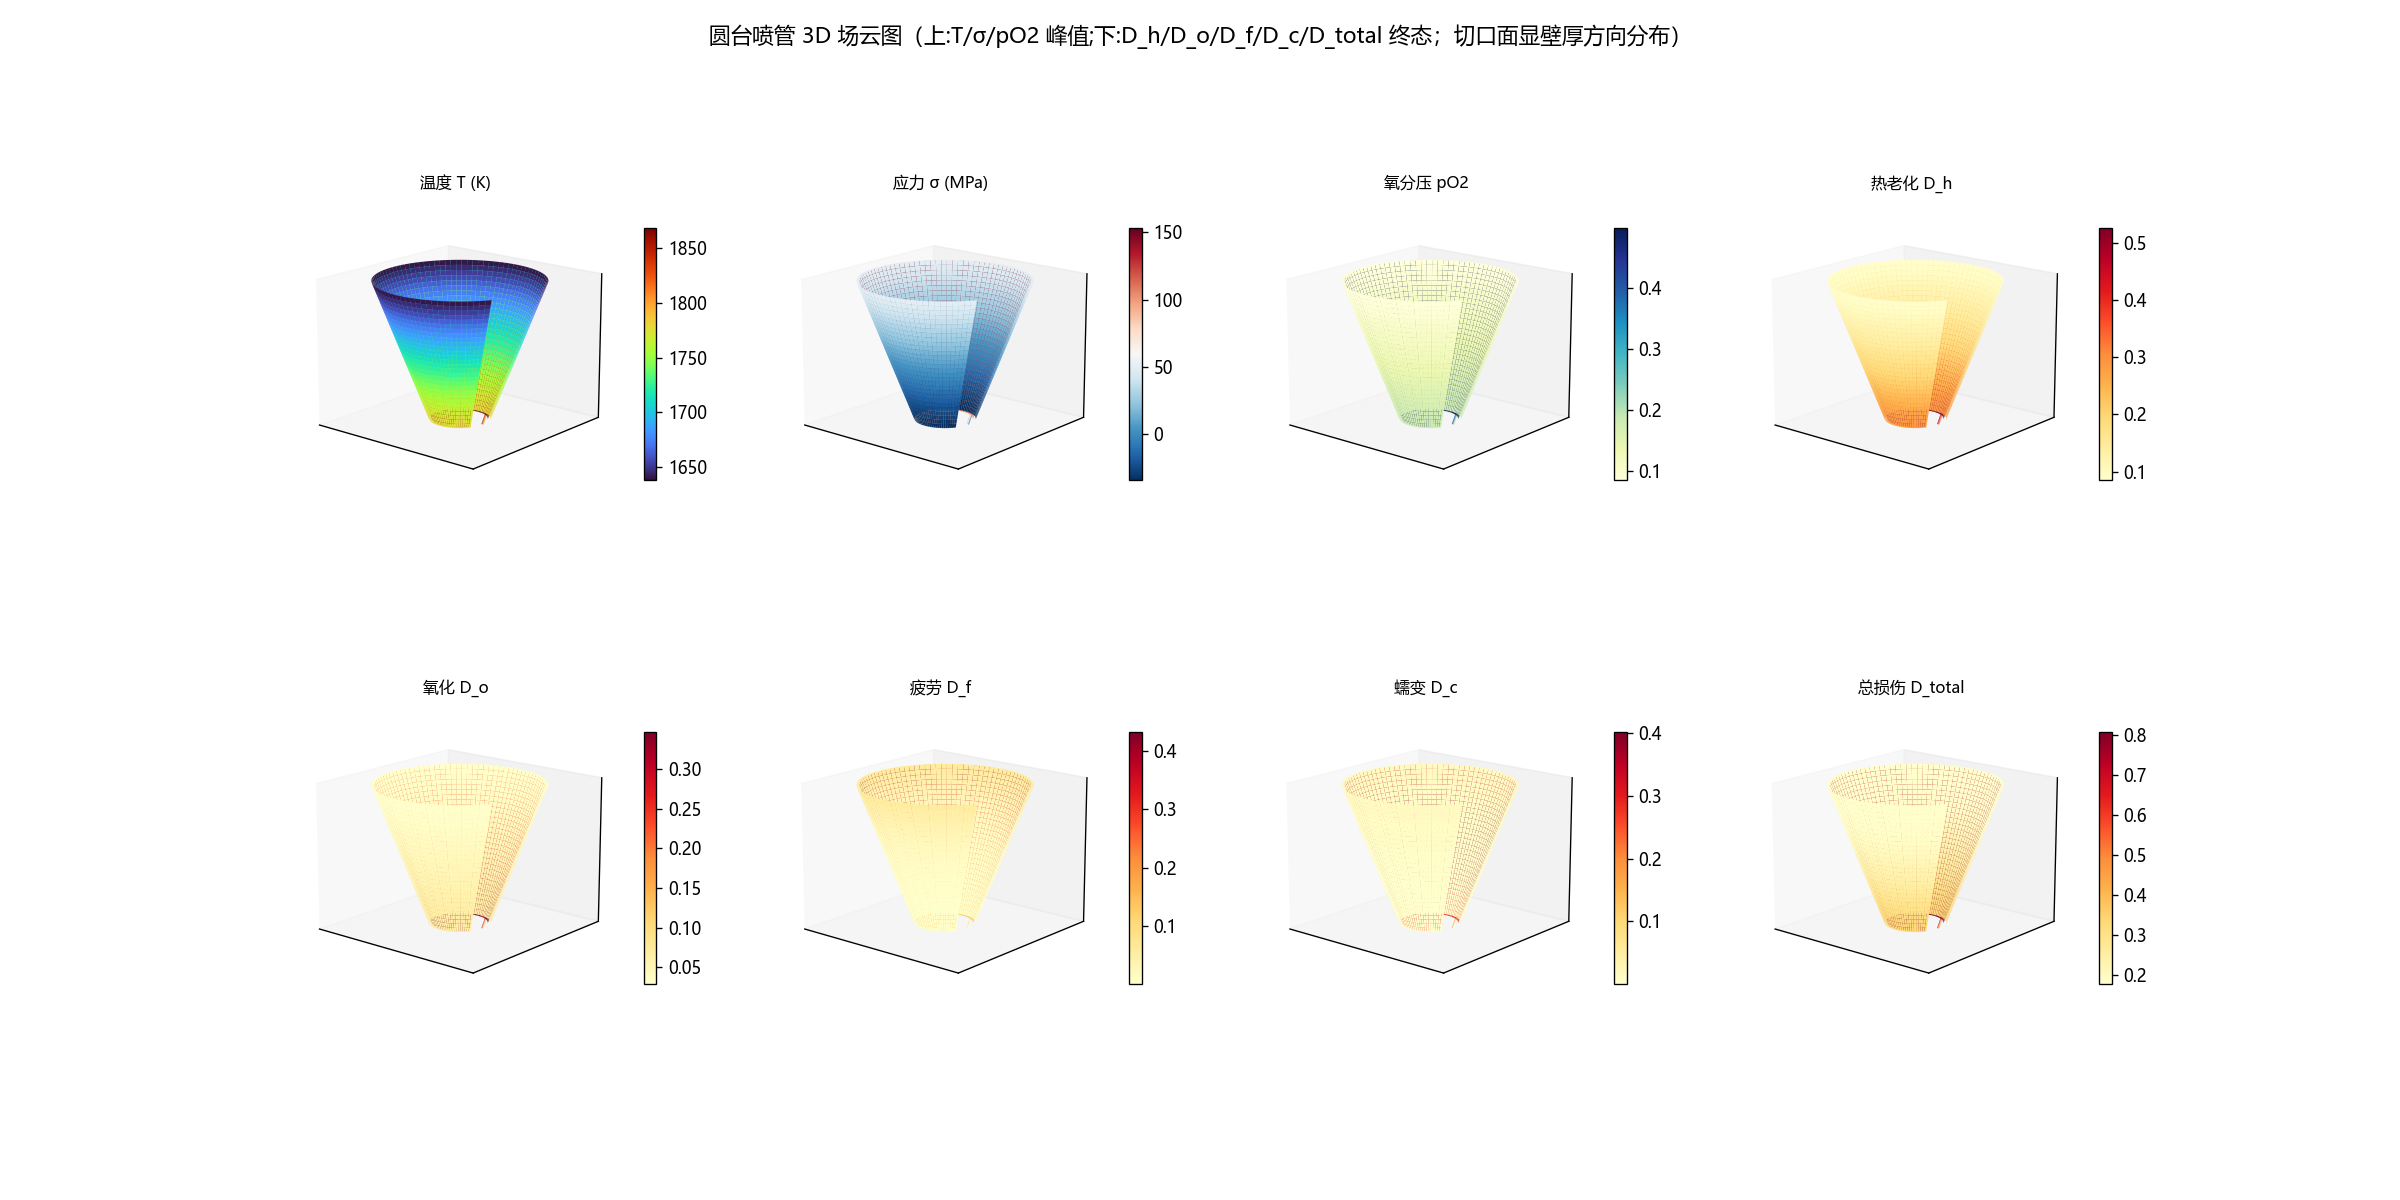
\includegraphics[width=\linewidth]{fig3d.png}
\caption{圆台喷管 3D 场云图。上：$T,\sigma,p_{O_2}$（峰值）；下：$D_h,D_o,D_f,D_c,D_{total}$（终态）。}\label{fig:3d}
\end{figure}

\section{讨论}
\textbf{与 universal resilience pattern 的关系。} 场方程中的拉普拉斯算子 $\nabla^2$ 即图拉普拉斯 $\sum_j A_{ij}(x_j-x_i)$，与 Gao 等\textsuperscript{3} 的 $\dot{x}_i=F(x_i)+\sum_j A_{ij}G(x_i,x_j)$（取 $G$ 为线性扩散、$A_{ij}$ 为网格邻接）完全一致——即场内部的空间耦合符合该韧性范式。差别在于：原文为单层单变量网络，本文为多场（多层）系统；场间跨场耦合以单向 $T/\sigma$ 驱动为主。

\textbf{求导精度与噪声可辨识性。} 交互项系数的恢复精度首先取决于时间求导的准确性：粗采样下 Savitzky--Golay 求导偏差经共因子 $\mathrm{arr}\cdot p_{O_2}$ 不均等地摊到各系数（小系数项尤甚），细采样（本文 $\Delta t{=}0.2$~s）下方能将误差压至 $\le 4\%$。这并非共线所致——设计矩阵条件数 $\sim 7$、方差膨胀因子 $\lesssim 10$，均属良性；直接以与积分一致的解析导数拟合可零误差命中真值，反证系数偏粗源于求导而非数据结构。在观测噪声下，含空间拉普拉斯算子的场×场项因算子放大噪声而比损伤×损伤项更难辨识——这是 SINDy 用于 PDE 系统的固有难点，也是真实强噪声场景须以状态估计/数据同化替代直接辨识的根本动因。饱和指数 $q$ 的可辨性则依赖于数据是否进入 $(1-D_f)^{-q}$ 的非线性区：深层非线性参数需深层（中后期）损伤数据方能辨识。

\textbf{面向真实强噪声与不完全观测的落地。} 火箭喷管极端高温、强振动环境下微观损伤参量极难测量、误差远大于本文的 $2\%$。SINDy 类方法对噪声敏感是通病，落地需引入状态估计与数据同化：以辨识所得机理方程为过程模型，用扩展/集合卡尔曼滤波（EnKF）或贝叶斯数据同化融合多保真数据（遥测时序 + 回收后超声无损检测 panel 数据），对状态与参数做联合后验估计；并以多保真分层（高保真 FEA 补密、低保真校准）缓解稀疏观测下导数估计的困难。

\textbf{局限与建模说明。} (i) 控制律为自设，本文为方法可行性验证，非真实机理发现；真实机理发现需真实/高保真数据、残差分析与样本外预测。(ii) 几何取薄壳近似（$h_{wall}/r\approx 3\%$--$10\%\ll 1$，见上），略去轴对称拉普拉斯曲率项 $(1/r)\partial_r$；如需完全轴对称可补回，对本薄壳改动量 $\lesssim 10\%$。(iii) 轴向两端取绝热 $\partial T/\partial z=0$（截断域的零通量边界），域内轴向温差由 $z$ 相关换热系数 $h_g(z)$ 产生；真实喷管两端与上下游结构有轴向导热，可改 Robin 边界作精化。(iv) 损伤变量 $D\in[0,1]$ 为损伤分数（$0$ 完好、$1$ 失效），演化设 $[0,0.9]$ 截断与 Paris 项 $(1-D_f)\ge 0.05$ 作数值 safeguards 以避开 $D\!\to\!1$ 的奇点；本仿真各损伤最大 $\approx 0.43$、$(1-D_f)>0.57$，二者均不触发，不影响辨识。(v) 图~\ref{fig:rec} 中 $0\%$ 噪声处的残余误差（$\sim 2\%$）即数值求导的方法误差下限，更高噪声级误差中超出该下限的部分方归因于观测噪声。

\section{结论}
(1) 在圆台喷管壁的合成耦合场上，多物理场耦合交互项（温度相关与应力调制氧扩散）与损伤内部交互项（应力助氧化、氧化–疲劳、氧化–蠕变等）均能被 SINDy 正确挖掘，无噪声下 $100\%$ 命中、$0$ 误选、系数误差 $\le 4\%$（前提为足够细的时间采样）；EIV 噪声下系数误差随噪声单调退化，损伤×损伤项较含拉普拉斯算子的场×场项稳健。
(2) 对真实场景不可靠已知的活化能与幂指数，SINDy-PI 的 profile 扫描可从数据辨识 $E_{a,d},E_{a,h},E_{a,o},E_{a,c}$ 与 $m,n,q$（均命中真值）；其中 $q$ 需仿真深化至损伤中后期非线性区方可辨识。naive 网格离散因共线失效，profile 为正确做法。
(3) 场内空间扩散耦合符合 universal resilience pattern；面向真实强噪声的落地路径为卡尔曼/贝叶斯数据同化 + 多保真融合。本研究为方法验证，真实机理发现待真实数据。

\section*{参考文献}
\begin{enumerate}\setlength{\itemsep}{1pt}
\item Molins, R. \textit{Oxidation effects on the fatigue crack growth behaviour of alloy 718 at high temperature}. \textbf{Acta Mater.} (1997).
\item Jadon, J. K. et al. \textit{Creep-fatigue interaction behavior of high temperature alloys: a review}. \textbf{Int. J. Fatigue} (2022).
\item Gao, J., Barzel, B. \& Barabási, A.-L. \textit{Universal resilience patterns in complex networks}. \textbf{Nature} \textbf{530}, 307--312 (2016).
\item Kaheman, K. et al. \textit{SINDy-PI: a robust algorithm for parallel implicit sparse identification of nonlinear dynamics}. \textbf{Proc. R. Soc. A} (2020).
\end{enumerate}

\end{document}
